\documentclass[ngerman]{gdb-aufgabenblatt}


\renewcommand{\Aufgabenblatt}{4}
\renewcommand{\Ausgabedatum}{Mi. 15.10.2014}
\renewcommand{\Abgabedatum}{Do. 31.10.2014}
\renewcommand{\Gruppe}{Cornelia Hofs�\ss{}, Aleksej Davletcurin, Sascha Marcel Hacker}
\renewcommand{\STiNEGruppe}{30}


\usepackage{listings} \lstset{numbers=left, numberstyle=\tiny, numbersep=5pt} \lstset{language=sql}



\begin{document}

\section{Relationenalgebra} 

\subsection*{a)}

$\pi_{Jahresgehalt}$(Job $\underset{JNR=Job}{\bowtie}$ Bewerbung $\underset{Bewerber=PNR}\bowtie$ ($\sigma_{Geb \geq \text{'1980-01-01'}}$(Person)))


\subsection*{b)}
$\pi_{Titel,Jahresgehalt}$(Job $\underset{JNR=Job}{\bowtie}$Bewerbung$\underset{Bewerber=PNR}\bowtie$Person$\underset{Heimat=LNR}\bowtie$($\sigma_{Name='Schweiz'}(Land)$))


\subsection*{c)} 
$\pi_{Vorname,Nachname}$(Personen$\bowtie(\pi_{PNR}(Personen)-\pi_{PNR}(Bewerber)) )$

\subsection*{d)}
Gebe das Geburtsdatum der Personen aus, deren Sachbearbeiter nach dem 31.12.1994 geboren worden sind.
\\

\section{Schemadefinition}
\subsection*{a)}
\lstinputlisting[frame=single,label=beispielcode,caption=Ein Beispiel]{create_table.sql}

\subsection*{b)}
Dadurch, dass die referentielle Integrit�t von Fremdschl�sseln nicht verz�gert am Ende der Trandaktion gepr�ft werden kann, k�nnen keine wechselseitigen Abh�ngigkeiten zwischen unterschiedlichen Tabellen aufgebaut werden. Wenn die Tablle Buch noch das Attribut Editor enthalten w�rde, das auf Person.Pid zeigt, dann k�nnen beide Tabellen erst einmal nicht erstellt werden, da sie voneinander abh�ngig sind. Eine L�sung w�re den Fremdschl�ssel mit Hilfe des Befehls alter table sp�ter einzuf�gen.


\subsection*{c)}
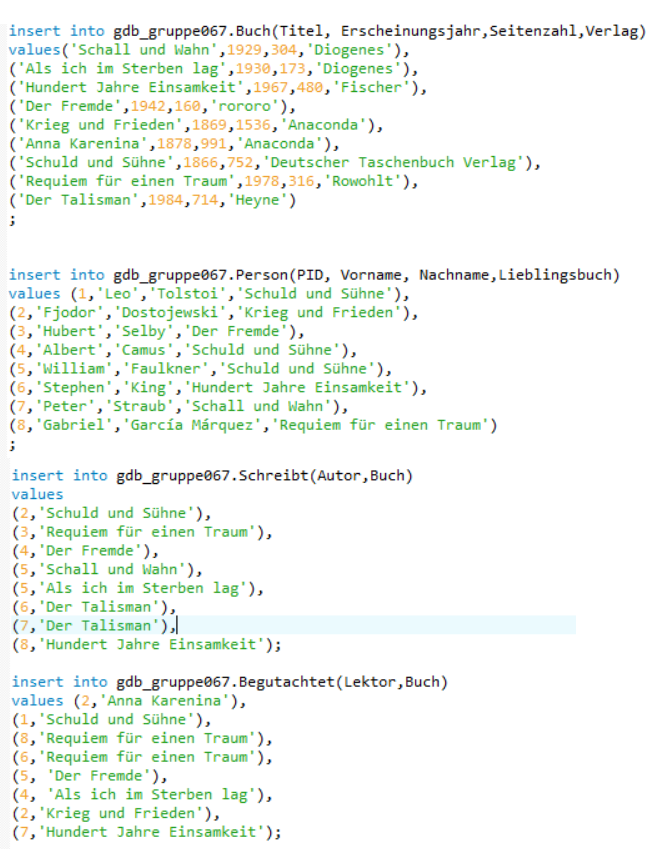
\includegraphics[]{insert_data}
\subsection*{d)}
\lstinputlisting[frame=single,label=beispielcode,caption=Ein Beispiel]{delete_peter.sql}


\section{SQL}
\subsection{a)}
\lstinputlisting[frame=single,label=beispielcode,caption=Ein Beispiel]{Anfragen1.sql}

\subsection{b)}
\lstinputlisting[frame=single,label=beispielcode,caption=Ein Beispiel]{Anfragen2.sql}

\subsection{c)}
\lstinputlisting[frame=single,label=beispielcode,caption=Ein Beispiel]{Anfragen3.sql}

\subsection{d)}
\lstinputlisting[frame=single,label=beispielcode,caption=Ein Beispiel]{Anfragen4.sql}
\section{Optimierung}


\end{document}
